249. \begin{figure}[ht!]
\center{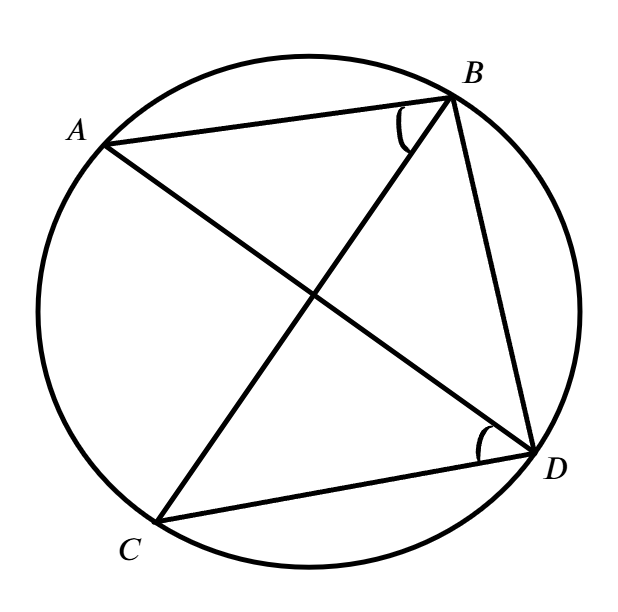
\includegraphics[scale=0.35]{g8-244.png}}
\end{figure}\\
Для того, чтобы равные углы $\angle ADC$ и $\angle CBA$ опирались на одну и ту же дугу $AC,$ точки должны быть расположены в следующем порядке: $A,\ B,\ D,\ C.$ Тогда дуга $AC=2\cdot 56^\circ=112^\circ,$ дуга $AB=2\cdot37^\circ=74^\circ,$ дуга $BDC=360^\circ-112^\circ-74^\circ=174^\circ,$ откуда $\angle BAC=\cfrac{1}{2}\cdot 174^\circ=87^\circ.$\\
